\section{Introduction}
\label{sec:intro}

We consider a rectangular area of dimension $W \times L$ subdivided into rectangular areas of dimension $w \times l$ each. We consider a cartesian reference system with $x$ pointing to the East and $y$ to the North as shown in figure~\ref{fig:area_subdivision}. The areas are indexed in left-to-right and bottom-up order.
For simplicity we assume that these dimensions are given as integers, that $l$ divides $L$ and $w$ divides $W$ (the input will be checked).
We use MPI as the implementation technology, so we decide to assign each country to a separate MPI process to improve the regularity of the program, while still not preventing multiple processes to be assigned to the same node.
\begin{figure}[h]
    \centering
    \begin{subfigure}[c]{0.7\textwidth}
    \begin{tikzpicture}
        % grid
        \draw[xstep=2, ystep=1] (0,0) grid (8,4);
        % axes
        \draw[->] (0,0) -- (8.25,0) node[right] {$x$};
        \draw[->] (0,0) -- (0,4.25) node[above] {$y$};
        \node[below left] at (0,0) {$0$};
        % country dimensions
        \draw[<->] (0,-.25) -- node[below] {$w$} (2,-.25);
        \draw[<->] (-.25,0) -- node[left] {$l$} (-.25, 1);
        % world dimensions
        \draw[<->] (0,-.75) -- node[below] {$W$} (8,-.75);
        \draw[<->] (-.75,0) -- node[left] {$L$} (-.75, 4);
        % country indices
        \matrix[matrix of nodes, inner sep=0, anchor=south west,
        nodes={minimum width=2cm, minimum height=1cm, inner sep=0, align=center}]{
            12 & 13 & 14 & 15 \\
                8 &  9 & 10 & 11 \\
                4 &  5 &  6 &  7 \\
                0 &  1 &  2 &  3 \\
        };
    \end{tikzpicture}
    \end{subfigure}
    \begin{subfigure}[c]{0.29\textwidth}
    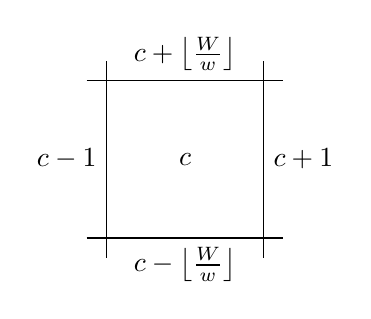
\begin{tikzpicture}
        \draw[step=2] (-.25,-.25) grid (2.25,2.25);
        \node           at (1,1) {$c$}; % center
        \node[above]    at (1,2) {$c + \left\lfloor \frac{W}{w} \right\rfloor$}; % north
        \node[right]    at (2,1) {$c + 1$}; % east
        \node[below]    at (1,0) {$c - \left\lfloor \frac{W}{w} \right\rfloor$}; % south
        \node[left]     at (0,1) {$c - 1$}; % west
    \end{tikzpicture}
    \end{subfigure}
    \caption{World subdivision into countries}
    \label{fig:area_subdivision}
\end{figure}

\noindent
Our program then considers a population $N$ and an initial number of infected individuals $I$ which are uniformly disitributed among the countries. \todo{consider explicit listing or random multinomial partitioning}

\paragraph{Motion}
The individuals will follow a linear motion with velocity $v$ (given in \si{m/s}), whose direction is randomly generated for each individual at the beginning of the simulation, and is kept also when moving from one country to another. When an individual is detected reaching (or surpassing) the world boundary it "bounces" onto it: the components of its speed perpendicular to the boundary will be inverted, as in figure~\ref{fig:boundary_bounce}.

\begin{figure}[h]
    \centering
    \begin{tikzpicture}[
        dot/.style={circle,fill,inner sep=1.25pt},
        >=stealth
    ]
        \node[dot, label=below:$p_s$] (p1) at (210:2) {};
        \node[dot,                  ] (p2) at (30:0) {};
        \node[dot,                  ] (p3) at (30:1) {};
        \node[dot, label=below:$p_d$] (p4) at (-30:1) {};
        \draw[-] (p1) -- (p2);
        \draw[->, dashed] (p2) -- (p3);
        \draw[->] (p2) -- (p4);
        \draw[-, very thick] (-2.5,0) -- (2.5,0);
        \draw[draw=none, pattern=north east lines] (-2.5,0) rectangle (2.5,.1);
    \end{tikzpicture}
    \caption{An individual bouncing on the world boundary}
    \label{fig:boundary_bounce}
\end{figure}

\paragraph{Infection and recovery}
If a subsceptible individual $i$ spends at least $t_{infection} = \SI{10}{min}$ at a distance $d_{ij}\leq d$ from an infected person $j$ it gets \emph{infected}, too.
After being infected for $t_{recovery} = \SI{10}{day}$ a person will become \emph{immune}, so it can't be infected or infect others. It will become subsceptible again after further $t_{immunity} = \SI{39}{days}$.

We only consider individuals in the same country when computing infections, in order to reduce the communication between processes. This means that if two individuals are closer than $d$ but in different countries, they won't be able to infect each other. This approximation should be acceptable in a realistic scenario where there are physical borders between countries and where $d$ is much smaller than the size of a country. However the "infection timer" of an individual is not reset when passing the border.

\paragraph{Simulation step}
The position and status of each individual is computed with a granularity of $t_{step}$ seconds, with no interpolation inbetween.
We compute periodic logs of the status of the population as soon as the end of each day has been surpassed, therefore we assume that $t_{step} \ll \SI{1}{day}$. Also, in a realistic scenario we should have $t_{step} \cdot v \ll w,l$ so that an individual cannot span a whole country in few steps.
The simulation ends when
\begin{enumerate*}[label=(\roman*)]
    \item $t \geq t_{target}$, or
    \item there are no infected people left
\end{enumerate*}.